% Chapter 4

\chapter{Extension of Wu et. al.'s algorithm toward social and dynamic navigation} % Main chapter title

\label{Chapter4} % For referencing the chapter elsewhere, use \ref{Chapter4}

\section{Discussion on the original hypotheses in the light of tests with the Pepper robot}\label{discussion_hypotheses_section}

\paragraph{} The pseudocode formulation \ref{appendix_basicmods_section} for this proposition is available in Appendix \ref{algorithms}.

\paragraph{} As eventually our experimental platform is to be a Pepper robot in the context of the Robocup@Home challenge that emulates a home setting, several hypotheses from the original algorithms have to be reconsidered:

\begin{itemize}
  \item \textbf{Initial knowledge of the environment} is partial, in that all static obstacles (i.e. objects that are not meant to be moved by any actor, like walls or very heavy furniture) have already been mapped. In the context of the Robocup@Home Challenge, participants are allowed to build such a map prior to the actual trials. This hypothesis is actually quite justified since in a home setting, it is very likely that the robot has undergone a configuration phase prior to its daily use, when it is provided with a manually drawn map of the home, or at least allowed to roam about and map the static obstacles. Having a map of static obstacles is very important for standard localization algorithms used in ROS, like \href{http://wiki.ros.org/amcl}{AMCL}, since they use this environment knowledge to compensate for odometry error.
  \item \textbf{Manipulation actions}, for the moment, are to be limited to pushes in a perpendicular direction to the obstacle's side being pushed. Given the many problematics related to grasping objects (e.g., appropriate positioning of the robot joints, keeping the robot balanced, ...), and the low power that can be delivered by Pepper's arms, it is best for a first iteration not to dwell on these.
  \item \textbf{Manipulation poses} are a key concept of manipulating obstacles, as we have shown in the previous chapter, and, contrary to the original algorithms we will explicitly explain our hypotheses as to them. Experimentations with the Pepper Robot (see Chapter \ref{Chapter5}) and carboard boxes as movable obstacles have shown that a good first approximation that guarantees quasi-systematic push manipulation successes are poses situated at the middle of the object's sides. This is, of course, supposing that we are only considering light objects with negligible friction against the ground, and with no other cinematic constraint than a plan-plan link between one of the obstacle's faces and the ground (a perfect plane).


  \item \textbf{Manipulation cost} A constant $pushCost$ has been used in the previously shown algorithm to allow weighting of the manipulation action in regard to a simple move action. Semantically, it makes more sense that this constant be related to the object (the difficulty of moving a specific object depending mainly on its physical properties), so we will store it as an obstacle attribute.
  \item \textbf{Manipulation possibility check} Checking whether a manipulation is possible or not is done by checking whether the area covered by the robot and the obstacle as they move together is in intersection with any other obstacle. As we limit our action set to pushes in a specific direction, this area can be defined as the convex hull containing both the robot's and the obstacle's polygonal representation at their initial and final pose. According to the existing litterature, we will call this the "safe-swept area" if no other obstacle is in intersection with it. In the pseudocode, this is done by the "GET-SAFE-SWEPT-AREA" method, which returns null if any obstacle is in intersection with the manipulation area. This area is saved as part of the plan so that when the plan is being executed, checking for a collision is as simple as checking if an obstacle appeared in this area (assuming our knowledge of the obstacle did not evolve in the mean time).
  \item \textbf{Obstacle discovery} As the robot approaches obstacles, their geometrical representation is updated according to what the robot's sensors can see. When executing a plan that includes the manipulation of an obstacle, said obstacle knowledge can actually evolve during the execution of the $c_{1}$ component, which is problematic for the preservation of optimality, since the obstacle's push poses may change (as a push pose has been defined with a dependency to the side's middle point). Therefore re-evaluation should not only be triggered if a new obstacle intersects with the current optimal plan, but also if the current optimal plan includes the manipulation of an obstacle and if said obstacle has changed in a way that makes the originally targeted $pushPose$ unavailable.
\end{itemize}

\subsection{Newly introduced notations and definitions}

\paragraph{\textbf{continue}}\label{continue_note} The \textbf{continue} statement returns the control to the beginning of the loop, and simply won't execute any of the remaining statements in the current iteration of the loop. This is done because a plan with a manipulation cannot exist without an empty $c_{1}$ component (i.e. the targeted push pose is not accessible).

\paragraph{COPY}\label{copy_note} Here, $p_{opt}.o$ is a copy of object $o$, and not the same object, so that when $o$ is updated because of the call to UPDATE-FROM-NEW-INFORMATION() on $I$, we can compare the difference between the two. We do the same for $p_{opt}.pushPose$ for the same reason. This allows us to trigger re-evaluation if the obstacle's push poses change and the one the robot aimed for no longer exists.

\paragraph{[], $\neq$ and $\bigcap$ operators}\label{operators_note} The [] operator is now also used as a short handle for "get the obstacle that corresponds in $\mathcal{O}$ that corresponds to the saved obstacle $p_{opt}.o$. The $\neq$ operator checks if the two states of the obstacle are the same or not (i.e, if the obstacle changed).

\paragraph{$\bigcap$}\label{area_intersect_note} The notation $\bigcap$ means here that we check for possible collisions between the swept area and any obstacle, since they may have changed.

\paragraph{Note on saving $translation$ in $p_{opt}$}\label{translation_note} The $translation$ necessary for manipulating the obstacle is saved to easily recompute the safe swept area when the obstacle changes.

\section{Social awareness through manipulation authorization consideration}\label{social_authorization_section}

\paragraph{} As shown in Chapter \ref{Chapter2}, to the best of our knowledge, the current NAMO litterature has never covered the idea of socially-aware navigation. Then, we must ask: what makes the action of moving an obstacle socially-aware or not?

\paragraph{} The first thing that comes to mind would be to consider that some objects are better not be moved because:

\begin{itemize}
  \item they are too fragile (e.g. flower pot),
  \item they have a high value in the human’s eye (e.g. a costly vase)
  \item they might cause the robot to break if it fails to move them properly (i.e. heavy or unstable objects)
  \item they are not supposed to be moved (i.e. exhibited objects)
  \item \dots
\end{itemize}

\paragraph{} Thus comes the notion of risk, either to the robot or to the manipulated objects. To mitigate this risk, we propose to modify our base algorithm presented in the first section of this chapter, so that an obstacle is not to be moved unless identified as belonging to a provided whitelist of "movable" obstacles.

\paragraph{} We will work under th hypothesis that if an obstacle is in the field of vision of the camera, the obstacle recognition will be perfect if it is in our whitelist of movable ostacles. If an obstacle is in the field of vision of the camera but is not recognized, we will assume that it is an obstacle that is not supposed to be moved. This is relatively safe hypothesis if identification of the obstacle's nature is done through computer vision, since it is one of the most efficient and most common ways to detect specific objects, by using trained neural networks for example\parencite{redmon_yolo9000:_2016}. However, robots come with all sort of sensors to detect obstacles: laser range finders, RGB(D) cameras, sonars, ... And often, as with Pepper (see Chapter \ref{Chapter5} for a description of Pepper's abilities), their fields of vision do not perfectly overlap: typically, an obstacle may be detected by the laser range finders or the sonars, but not be within the field of vision of the RGB(D) camera, because it is in its blind spot or simply too close or too far away. This creates a situation where the robot knows an obstacle is there, but cannot definitely categorize it as "movable" or "unmovable" since it is not in the camera's field of vision.

\paragraph{} Then, it means that the algorithm must be adapted not only to manage the fact that an object should be considered for manipulation if and only if it is not deemed "unmovable", but also to eventually adapt the robot's trajectory \textbf{in an optimal way} so that an "unidentified" / "potentially movable" object can be identified with certainty before engaging with the manipulation procedure.

\paragraph{} For that, when we evaluate an obstacle, we first check whether the obstacle has already been identified or not (Alg. \ref{alg:04-custom-observation-planforobstacle}, lines \ref{lst:line:identified_1} and \ref{lst:line:identified_2}). If it has been identified as "movable", the algorithm does not change. If it has been identified as "unmovable", the obstacle evaluation routine simply stops before actually evaluating. And finally, if the evaluated obstacle is "unidentified":

\begin{itemize}
  \item The $c_{1}$ plan component that goes from the current robot pose to the push pose is evaluated just as before (Alg. \ref{alg:04-custom-observation-planforobstacle}, line \ref{lst:line:c1_computation}),
  \item If a pose comprised in the computed $c_{1}$ component allows the camera field of vision to encompass the obstacle's currently known geometry, keep the precomputed $c_{1}$ component (Alg. \ref{alg:04-custom-observation-planforobstacle}, lines \ref{lst:line:keep_c1_1} to \label{lst:line:keep_c1_2}, and Alg. \ref{alg:04-custom-observation-simple-checkpath}),
  \item Else we must find a shortest path component $c_{0}$ from the current robot pose to an "observation pose" where we know we can identify the obstacle as "movable" or "unmovable" with certainty and recompute $c_{1}$ as the path from this "observation pose" to the push pose. Recomputing is done in the COMPUTE-C0-C1 method (Alg. \ref{alg:04-custom-observation-simple-compute01c1}), which is a baseline, naive implementation where we iterate over every "observation pose" to compute a path for $c_{0}$ and $c_{1}$ and only keep the shortest total path (this is illustrated in Figure \ref{fig:observation_example}). If neither $c_{0}$ or $c_{1}$ components are found, then stop evaluating plans for the current push pose (Alg. \ref{alg:04-custom-observation-planforobstacle}, lines \ref{lst:line:noc0c1_1} to \ref{lst:line:noc0c1_2}). Since the robot's obstacle representation may change as the robot approaches it, the condition favors paths combinations with an observation point that is closest to the current robot's pose, so that there are more chances for the robot to still have a valid observation pose in the current plan avoiding the need to recompute a plan in some cases.
  \item The observation poses are updated in the same way that push poses are: automatically, whenever an obstacle is updated. These poses are situated at every grid point for which the field of vision of the robot sensor(s) dedicated to obstacle recognition covers the entire known obstacle's geometry. Though the presented algorithm is not affected by the representation of the identification sensor's field of vision, in our experimentation, we will consider a single RGB(D) camera, and approximate its field of vision by the difference between a circular sector and a disk of same center, coincident with the robot's center, which is an acceptable representation for the Pepper robot capabilities. The circular sector has a radius $r_{max}$, central angle $\theta$ and is equally partitioned around the robot's orientation direction line. The disk has a radius $r_{min}$. This is illustrated in Figure \ref{fig:robot_camera_fov}.
\end{itemize}

\begin{figure}[H]
  \centering
  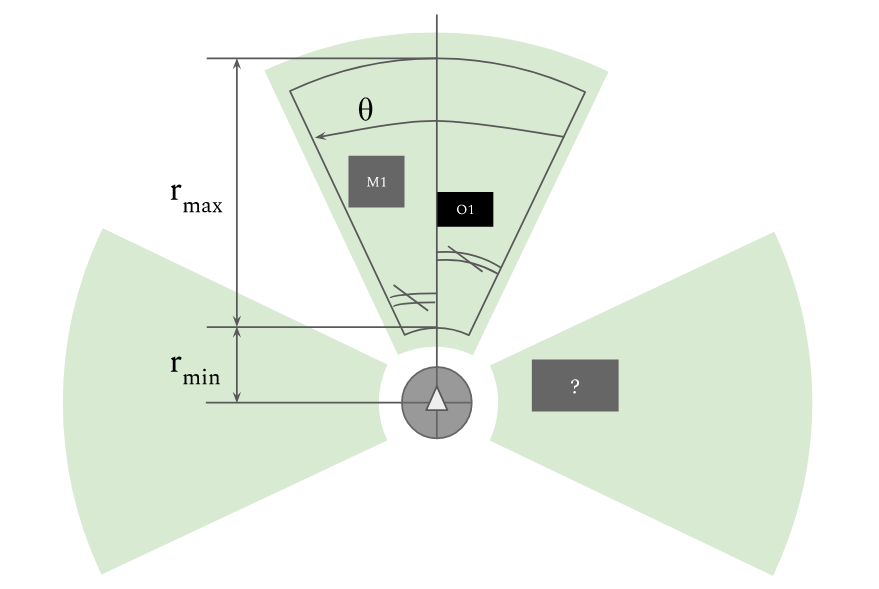
\includegraphics[width=10cm]{Figures/Observation_Proposition/Robot_Camera_FOV.png}
  \caption{Illustration of the field of vision of the different sensors of the Pepper robot: the green circular sectors correspond to laser sensors that only provide information about the obstacle's geometry. The grey line sector is the FOV of the camera used for identification. We can see that movable obstacle M1 and unmovable obstacle O1 have been identified but another obstacle "?" is yet to be.}
  \label{fig:robot_camera_fov}
\end{figure}

\paragraph{}In \ref{fig:observation_01}, the robot is in a situation where its laser sensors (green) have detected an obstacle to its left, but the obstacle has not yet been identified. When evaluating possible manipulation plans, the robot will need to build a $c_{1}$ component to every push pose of the obstacle (like the one in grey dots on the right). However, it is clear that here, the robot is too close, and the $c_{1}$ component (black arrow) being the shortest path to the push pose, it will not allow the camera FOV to encompass the obstacle, thus preventing identification. In \ref{fig:observation_02}}, we can see an example application of our proposition that would allow the robot to find an optimal plan in two components $c_{0}$ (in blue) and $c_{1}$ (in green) that allows it to identify the obstacle.

\begin{figure}[H]
\centering
\begin{subfigure}{.48\textwidth}
  \centering
  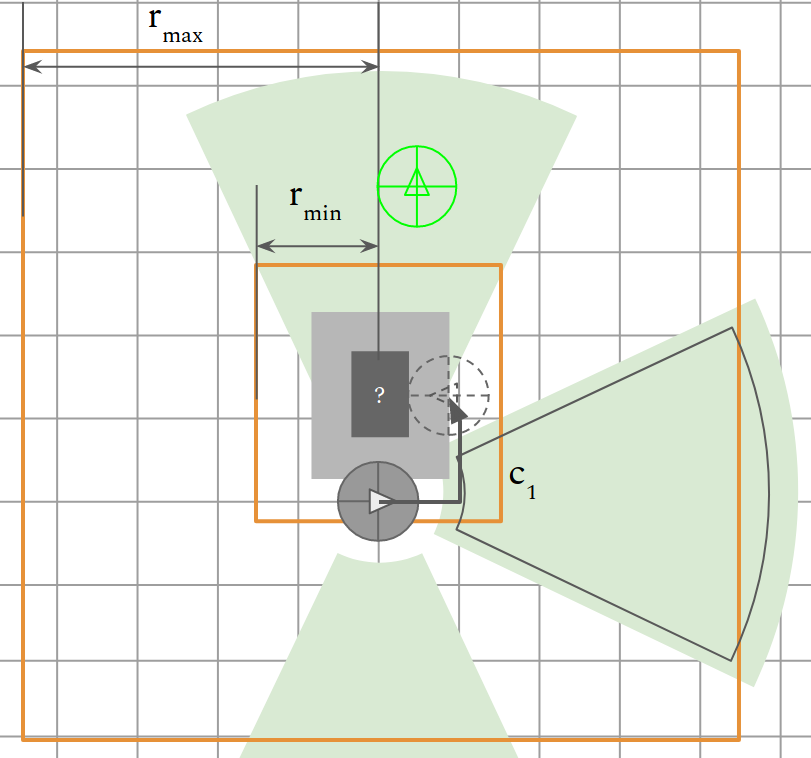
\includegraphics[width=\linewidth]{Figures/Observation_Proposition/Observation_01.png}
  \caption{Initial situation: goal is the green disk with a triangle, and the zone where the robot could potentially see the obstacle is delimited by the area between the two orange rectangles. The observation poses are situated at every grid intersection within the area and are orientated toward the robot's center.}
  \label{fig:observation_01}
\end{subfigure}\hspace*{\fill}
\begin{subfigure}{.48\textwidth}
  \centering
  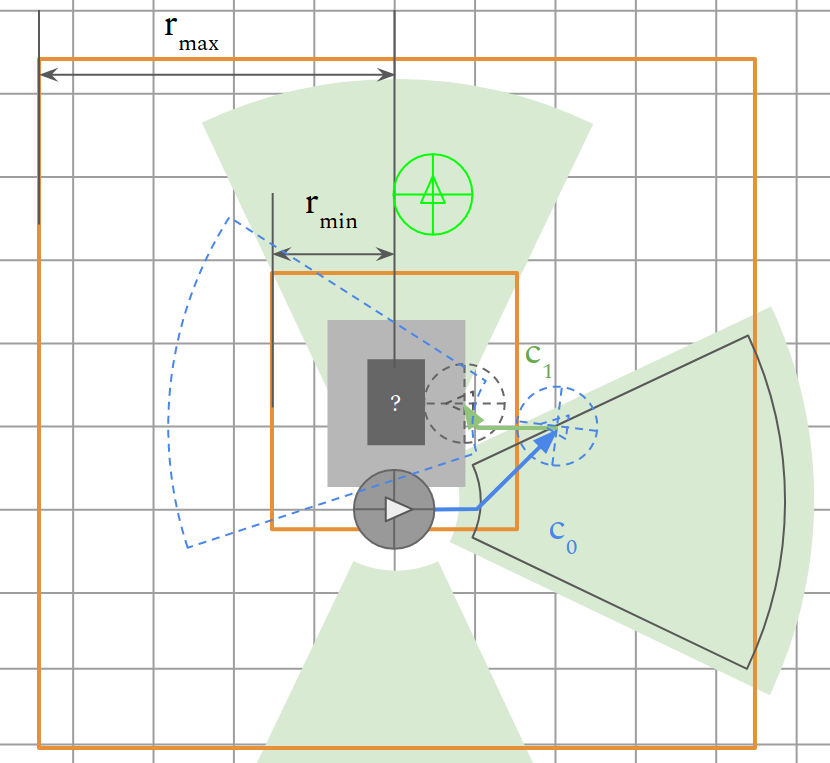
\includegraphics[width=\linewidth]{Figures/Observation_Proposition/Observation_02.png}
  \caption{The intermediary pose that is the goal of $c_{0}$ is the blue disk, and we can see that the camera FOV (blue dotted circular sector) would then encompasses the obstacle, allowing for an identification decision.}
  \label{fig:observation_02}
\end{subfigure}
\caption{Example situation showing the use of the $c_{0}$ component.}
\label{fig:observation_example}
\end{figure}

\paragraph{} In order to keep our local optimality property, we also modified the main execution loop, see Algorithm \ref{alg:04-custom-observation-makeandexecuteplan} (changes are highlighted in green). Basically, we added a check after the robot gets the next step to be executed and its parent plan component: if the currently considered optimal plan implies moving an obstacle that hasn't been identified yet, the next step component is $c_{0}$ or $c_{1}$, and the obstacle has changed since the previous environment observation in a way that the current plan does not allow to identify it anymore, then we must not execute the next step but re-evalutate the plan, since it may no longer be optimal.

\paragraph{Optimized version} It is obvious that the COMPUTE-C0-C1 method can be optimized in terms of execution time, in an analogous way the original algorithm did, by reducing calls to A*. A heuristic cost defined as the sum of the euclidian distance between the current pose and observation pose, and euclidean distance between observation pose and currently evaluated push pose is computed for every observation pose (Alg. \ref{alg:04-custom-observation-optimized-compute01c1}, lines \ref{lst:line:occ_heur_1} to \ref{lst:line:occ_heur_1}), and allows to order them in a list $euPosesCostL$, sorted by ascending heuristic cost. The list is then traversed until the heuristic cost of the current element is greater than the current optimal cost of $c_{0}$ + $c_{1}$ likely allowing not to evaluate many observation points (Alg. \ref{alg:04-custom-observation-optimized-compute01c1}, lines \ref{lst:line:traverse_eu_1} to \ref{lst:line:traverse_eu_2}).

\paragraph{Future work} It would be interseting to do a performance comparison between the two versions of our COMPUTE-C0-C1 method, and maybe further optimizing it by using a fitter algorithmic approach than calling A* many times. For example, using Dijkstra's algorithm to first get the path to all observation points in a single graph search rather than many could lead to better performance, especially if there is a great number of observation poses to check.

\section{Social awareness through placement consideration}\label{social_appendix_placement_section}

\paragraph{} Now that we have a basic capability for the algorithm to deal with obstacles depending on whether they have been explicitly defined as "movable" or not, we have an answer to the question "what obstacles can be moved in a socially-aware manner?". But then, this only characterizes the obstacle itself, and not the action of moving it. When moving an obstacle, not only do we have to consider the obstacle we are moving, but also where we are moving it: it would definitely not be acceptable for a robot to move an obstacle in an area where it would impair other actor's movements (e.g., by blocking an entryway, a corridor, ...).

\paragraph{} Handling this, while keeping the local optimality property, can be achieved by redefining the cost of a plan not just as being dependent on the distance, time or energy, but also on the compliance to the social rule of not placing obstacles in specific places that we will call "social cost".

\paragraph{} In this proposition, we define "socially forbidden/allowed" areas as cells of a 2D grid costmap, that have a value comprised between an arbitrary minimal integer value ALLOWED\_VALUE and maximal value FORBIDDEN\_VALUE, in an analogous way to the costmap_2d of ROS\footnote{ROS documentation page: \url{http://wiki.ros.org/costmap_2d}}. Since an obstacle may occupy several points, the total cost of moving an obstacle to some place is expressed as the normalized sum of the costs of covering each point (See Alg. \ref{alg:05-custom-placement-getocccost}, line \ref{lst:line:sumocccost}). If a cell is associated with the minimal value then it means that there is no particular wish to avoid covering it with an obstacle, not affecting the total cost (Alg. \ref{alg:05-custom-placement-getocccost}, lines \ref{lst:line:noocccost_1} to \ref{lst:line:noocccost_2}). On the contrary, if it is associated with the maximal value, no obstacle should ever be placed over it, raising the total cost to $+\infty$ (Alg. \ref{alg:05-custom-placement-getocccost}, lines \ref{lst:line:maxocccost_1} and \ref{lst:line:maxocccost_2}). This total cost is then simply added in the computation of the cost of the $c_{2}$ plan component as a product (Alg. \ref{alg:05-custom-placement-planforobstacle}, highlighted lines).

\paragraph{Future work} Though here, we limit ourselves to a static costmap of "socially forbidden" areas, nothing actually stands in the way of updating it according to the data the robot collects about the environment. This could allow to detect inappropriate areas for leaving obstacles that depend on other moving or movable obstacles (e.g., behind a chair, around a wheeled table, ...). This could also, if the algorithm were also modified to handle autonomously moving objects, allow to dynamically attribute a higher placement cost in areas where other agents like humans are about to pass through (for example, by building upon existing work, as in \parencite{jumel_mapping_2017}, where a method for mapping the likelihood of encoutering humans in an environment is described): we would not want the robot to put an obstacle right in front of a human or a robot minding their own businesses.

\section{Taking dynamic obstacles into account}\label{dynamic_section}

\paragraph{} A big missing piece in the existing NAMO algorithms is that they often, as is the case with the original one we are building upon here, operate under the assumption that there are no other autonomous agents around. Therefore, an obstacle cannot move of its own volition. For the home environment setting we are aiming for, this is only acceptable if the inhabitants are not here during the robot's activities, and neither pets or other robots are. However, one of the main points of having a service robot at home is to actually interact with it. Therefore, we must at least adapt the algorithm not to enter in collision with a moving obstacle (which it would in its current state since it only invalidates a plan when \textbf{new} obstacles are found to be intersected with), and keep making locally optimal decisions.

\paragraph{} For that, it is only necessary to modify the main execution loop, since the state of the robot's knowledge about the environment only ever changes here. First thing to do is to now consider all obstacles when checking for an intersection with the current plan: $\mathcal{O}_{new}$ is no longer useful, thus removed.

\paragraph{} To keep local optimality, we chose the simplest approach: whenever an obstacle is detected as having moved, we trigger a plan re-evaluation, though we don't invalidate the current one if it is still valid (according to the same criteria as in Algorithm  \ref{alg:03-custom-basicmods-makeandexecuteplan}). For that, we assume that, when updated, the world state representation $I$ saves in a list $I.movedObstacles$ the obstacles that have moved since its last update by checking whether they don't occupy some of the space they previously occupied. If this list is not empty, then we must trigger a re-evaluation. Also, since in terms of computation time, the plan evaluation is by far the longest element, if we just went through it, then we do not directly execute the plan but go back to the beginning of the loop and check the environment again. If no obstacles moved since then, the plan will be executed. Otherwise, it will be recomputed. This way, local optimality is always guaranteed.

\paragraph{Future work} While the current proposition retains local optimality, if obstacles are constantly moving around the robot, then it will never budge, always recomputing plans, until its the environment in its field of vision stops moving: this is known as the "robot freezing problem" \parencite{trautman_unfreezing_2010}. Furthermore, autonomously moving obstacles follow trajectories that can usually be predicted, at least in a short time window: it may not be interesting to invalidate the current plan and/or trigger a plan re-evaluation if an obstacle just passes by the robot in a way that would not affect the optimality of its plan. Incorporating existing work on taking obstacle trajectory predictions into account will be the object of future study. It may also be interesting to study how to merge the existing NAMO algorithms with an existing algorithm for navigation among dynamic obstacles like D* or D*Lite in a way that actually takes advantage of the incremental building of knowledge of these algorithms.

\section{Algorithm proposition}\label{merged_proposition_section}

\paragraph{} The final algorithm proposition is a merge of the previously presented individual propositions. It consists of Algorithms \ref{alg:07-custom-merge-makeandexecuteplan-part1}, \ref{alg:02-levihn-makeplan} and \ref{alg:07-custom-merge-optimized-planforobstacle-part1} and the newly created subroutines \ref{alg:04-custom-observation-optimized-compute01c1}, ref{alg:04-custom-observation-simple-checkpath} and \ref{alg:05-custom-placement-planforobstacle}. All these can be found in the Appendix \ref{algorithms}.
